\documentclass[10pt]{article}
\usepackage[utf8]{inputenc}
\usepackage[T1]{fontenc}
\usepackage{amsmath}
\usepackage{amsfonts}
\usepackage{amssymb}
\usepackage[version=4]{mhchem}
\usepackage{stmaryrd}
\usepackage{bbold}
\usepackage{graphicx}
\usepackage[export]{adjustbox}
\graphicspath{ {./images/} }

\begin{document}
\section*{Lecture hours 19-20}
\section*{Definitions and Theorems}
Definition (Coordinates of a vector ).\\
If we have a basis of $\mathbb{R}^{n}, \mathcal{B}=\left\{\vec{v}_{1}, \vec{v}_{2}, \ldots, \vec{v}_{n}\right\}$ and $\vec{x} \in \mathbb{R}^{n}$, so $\vec{x}=c_{1} \vec{v}_{1}+\cdots+c_{n} \vec{v}_{n}$, for some $c_{1}, \ldots c_{n} \in \mathbb{R}$. We define the coordinates of $\vec{x}$ in the basis $\mathcal{B}$ as

$$
[\vec{x}]_{\mathcal{B}} \stackrel{\text { def }}{=}\left[\begin{array}{c}
c_{1} \\
\vdots \\
c_{n}
\end{array}\right]
$$

Definition (Change of basis matrix ).\\
Let $\mathcal{B}=\left\{\vec{v}_{1}, \vec{v}_{2}, \ldots, \vec{v}_{n}\right\}$ be a basis of $\mathbb{R}^{n}$. We call the matrix $S=\left[\vec{v}_{1}, \ldots, \vec{v}_{n}\right]$ the change of basis matrix of basis $\mathcal{B}$.

For any $\vec{x} \in \mathbb{R}^{n}$ we have

$$
\vec{x}=S[\vec{x}]_{\mathcal{B}}
$$

So, if we have to find the coordinates $[\vec{x}]_{\mathcal{B}}$ we compute

$$
[\vec{x}]_{\mathcal{B}}=S^{-1} \vec{x} .
$$

Note that

\begin{itemize}
  \item If $\mathcal{B}=\left\{\vec{e}_{1}, \vec{e}_{2}, \ldots, \vec{e}_{n}\right\}$ (the standard basis), we have $[\vec{x}]_{\mathcal{B}}=\vec{x}$.
\end{itemize}

Problem 37 (Coordinates). Let $\mathfrak{B}$ be the basis of $\mathbb{R}^{4}$ given by

$$
\mathfrak{B}=\left\{\left[\begin{array}{l}
3 \\
1 \\
1 \\
1
\end{array}\right],\left[\begin{array}{l}
1 \\
1 \\
1 \\
0
\end{array}\right],\left[\begin{array}{l}
1 \\
1 \\
0 \\
0
\end{array}\right],\left[\begin{array}{l}
1 \\
0 \\
0 \\
0
\end{array}\right]\right\}
$$

Find the coordinates for vector

$$
\vec{v}=\left[\begin{array}{l}
4 \\
3 \\
2 \\
1
\end{array}\right]
$$

in the basis $\mathfrak{B}$.

Solution 37 (Coordinates) Let $E=\left\{\vec{e}_{1}, \vec{e}_{2}, \vec{e}_{3}, \vec{e}_{4}\right\}$ be the standard basis of $\mathbb{R}^{4}$. Define

$$
S=\left[\begin{array}{llll}
3 & 1 & 1 & 1 \\
1 & 1 & 1 & 0 \\
1 & 1 & 0 & 0 \\
1 & 0 & 0 & 0
\end{array}\right]
$$

The change of basis matrix from the standard basis $E$ to basis $\mathfrak{B}$ is given by

$$
S^{-1}=\left[\begin{array}{cccc}
0 & 0 & 0 & 1 \\
0 & 0 & 1 & -1 \\
0 & 1 & -1 & 0 \\
1 & -1 & 0 & -2
\end{array}\right]
$$

Thus

$$
[\vec{v}]_{\mathfrak{B}}=S^{-1}[\vec{v}]_{E}=S^{-1} \vec{v}=\left[\begin{array}{c}
1 \\
1 \\
1 \\
-1
\end{array}\right] .
$$

Problem 38 (Coordinates). In this problem we will be working with the following bases of $\mathbb{R}^{3}$ :

$$
\mathfrak{B}=\left\{\left[\begin{array}{c}
-3 \\
2 \\
-3
\end{array}\right],\left[\begin{array}{c}
1 \\
-1 \\
-1
\end{array}\right],\left[\begin{array}{l}
5 \\
4 \\
9
\end{array}\right]\right\}, \quad E=\left\{\left[\begin{array}{l}
1 \\
0 \\
0
\end{array}\right],\left[\begin{array}{l}
0 \\
1 \\
0
\end{array}\right],\left[\begin{array}{l}
0 \\
0 \\
1
\end{array}\right]\right\}, \quad \mathfrak{D}=\left\{\left[\begin{array}{l}
1 \\
2 \\
1
\end{array}\right],\left[\begin{array}{c}
-1 \\
2 \\
-1
\end{array}\right],\left[\begin{array}{l}
1 \\
1 \\
3
\end{array}\right]\right\}
$$

\begin{enumerate}
  \item Find the change of basis matrix from basis $\mathfrak{B}$ to the standard basis $E$.
  \item Find the change of basis matrix from the standard basis $E$ to basis $\mathfrak{D}$.
  \item Find the change of basis matrix from basis $\mathfrak{B}$ to basis $\mathfrak{D}$.
\end{enumerate}

Solution 38 (Coordinates) Define

$$
S=\left[\begin{array}{ccc}
-3 & 1 & 5 \\
2 & -1 & 4 \\
-3 & -1 & 9
\end{array}\right], \quad \text { and } \quad R=\left[\begin{array}{ccc}
1 & -1 & 1 \\
2 & 2 & 1 \\
1 & -1 & 3
\end{array}\right]
$$

\begin{enumerate}
  \item The change of basis matrix from basis $\mathfrak{B}$ to basis $E$ is given by S .
  \item The change of basis matrix from basis $E$ to basis $\mathfrak{D}$ is given by
\end{enumerate}

$$
R^{-1}=\frac{1}{8}\left[\begin{array}{ccc}
7 & 2 & -3 \\
-5 & 2 & 1 \\
-4 & 0 & 4
\end{array}\right]
$$

\begin{enumerate}
  \setcounter{enumi}{2}
  \item The change of basis matrix from basis $\mathfrak{B}$ to basis $\mathfrak{D}$ is given by
\end{enumerate}

$$
R^{-1} S=\frac{1}{8}\left[\begin{array}{ccc}
7 & 2 & -3 \\
-5 & 2 & 1 \\
-4 & 0 & 4
\end{array}\right]\left[\begin{array}{ccc}
-3 & 1 & 5 \\
2 & -1 & 4 \\
-3 & -1 & 9
\end{array}\right]=\left[\begin{array}{ccc}
-1 & 1 & 2 \\
2 & -1 & -1 \\
0 & -1 & 2
\end{array}\right]
$$

What are the columns of $R^{-1} S$ in terms of coordinates?\\
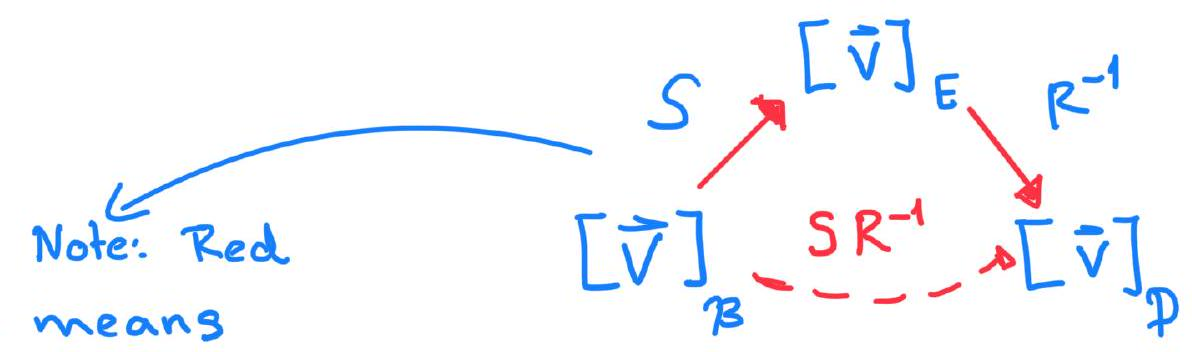
\includegraphics[max width=\textwidth, center]{2024_12_26_e97821198783008ca6d9g-3}

$$
\bar{v}=[\dot{v}]_{E}=S[\bar{v}]_{93}
$$

(matrix multiplication).

Problem 39 (Coordinates for linear transformations). In this problem we will be working with the same bases of $\mathbb{R}^{3}$ as in Problem 38:\\
$\mathfrak{B}=\left\{\left[\begin{array}{c}-3 \\ 2 \\ -3\end{array}\right],\left[\begin{array}{c}1 \\ -1 \\ -1\end{array}\right],\left[\begin{array}{l}5 \\ 4 \\ 9\end{array}\right]\right\}, \quad E=\left\{\left[\begin{array}{l}1 \\ 0 \\ 0\end{array}\right],\left[\begin{array}{l}0 \\ 1 \\ 0\end{array}\right],\left[\begin{array}{l}0 \\ 0 \\ 1\end{array}\right]\right\}, \quad \mathfrak{D}=\left\{\left[\begin{array}{l}1 \\ 2 \\ 1\end{array}\right],\left[\begin{array}{c}-1 \\ 2 \\ -1\end{array}\right],\left[\begin{array}{l}1 \\ 1 \\ 3\end{array}\right]\right\}$\\
. Let $T: \mathbb{R}^{3} \rightarrow \mathbb{R}^{3}$ be the linear transformation defined by

$$
T \vec{v}=A \vec{v}
$$

where

$$
A=\left[\begin{array}{lll}
3 & 1 & 1 \\
1 & 1 & 1 \\
1 & 1 & 0
\end{array}\right]
$$

Find the matrix $[T]_{\mathfrak{B}}^{\mathfrak{D}}$.\\
Remember that the matrix $[T]_{\mathfrak{B}}^{\mathfrak{D}}$ satisfies:

$$
[T \vec{v}]_{\mathfrak{D}}=[T]_{\mathfrak{B}}^{\mathfrak{B}}[\vec{v}]_{\mathfrak{B}}
$$

for any $\vec{v} \in \mathbb{R}^{3}$.

Solution 39 (Coordinates for linear transformations)\\
Define

$$
S=\left[\begin{array}{ccc}
-3 & 1 & 5 \\
2 & -1 & 4 \\
-3 & -1 & 9
\end{array}\right], \quad \text { and } \quad R=\left[\begin{array}{ccc}
1 & -1 & 1 \\
2 & 2 & 1 \\
1 & -1 & 3
\end{array}\right]
$$

Take any $\vec{v} \in \mathbb{R}^{3}$.\\
To find $[T]_{\mathfrak{B}}^{\mathfrak{D}}$ take the following steps:

\begin{enumerate}
  \item Since we start with $[\vec{v}]_{\mathfrak{B}}$, we first need to change to standard basis coordinates: $[\vec{v}]_{E}=S[\vec{v}]_{\mathfrak{B}}$.
  \item We know A is the matrix representation of T in the standard basis coordinates. Thus $[T \vec{v}]_{E}=A S[\vec{v}]_{\mathfrak{B}}$.
  \item Finally, we need to transform vector $A S \vec{v}$ from standard coordinates to $\mathfrak{D}$ coordinates. That is $[T \vec{v}]_{\mathfrak{B}}=R^{-1} A S[\vec{v}]_{\mathfrak{B}}$. Therefore $[T]_{\mathfrak{B}}^{\mathfrak{M}}=R^{-1} A S$.
\end{enumerate}

$$
\begin{aligned}
& {[\bar{v}]_{E} \xrightarrow{A}[T \stackrel{\rightharpoonup}{v}]_{E}} \\
& s \uparrow \mid R^{-1} \\
& \left.[\bar{v}]_{B} R^{-1} A S \rightarrow T T_{V}\right]_{D}
\end{aligned}
$$

Problem 40 (Elementary matrices). Write the matrix

$$
A=\left[\begin{array}{ccc}
1 & 0 & -1 \\
0 & -2 & 2 \\
-1 & 1 & 1
\end{array}\right]
$$

as a product of elementary row matrices. Use your expression to find $A^{-1}$.

Solution 40 (Elementary matrices) By Gauss-Jordan elimination, we have $E_{5} E_{4} E_{3} E_{2} E_{1} A=$ $I$, where

$$
\begin{aligned}
& E_{1}=\left[\begin{array}{lll}
1 & 0 & 0 \\
0 & 1 & 0 \\
1 & 0 & 1
\end{array}\right], \\
& E_{2}=\left[\begin{array}{lll}
1 & 0 & 0 \\
0 & 1 & 2 \\
0 & 0 & 1
\end{array}\right], \\
& E_{3}=\left[\begin{array}{lll}
1 & 0 & 0 \\
0 & 0 & 1 \\
0 & 1 & 0
\end{array}\right], \\
& E_{4}=\left[\begin{array}{ccc}
1 & 0 & 0 \\
0 & 1 & 0 \\
0 & 0 & 1 / 2
\end{array}\right], \\
& E_{5}=\left[\begin{array}{lll}
1 & 0 & 1 \\
0 & 1 & 0 \\
0 & 0 & 1
\end{array}\right] .
\end{aligned}
$$

$A=E_{1}^{-1} E_{2}^{-1} E_{3}^{-1} E_{4}^{-1} E_{5}^{-1}$. We have $A^{-1}=E_{5} E_{4} E_{3} E_{2} E_{1}$.


\end{document}